\documentclass[../main.tex]{subfiles}
\graphicspath{{\subfix{../diagrams/}}}


\begin{document}
\subsection{Sequence diagrams}
\subsubsection{Preparing order}


One of the most important activities in the system is preparing and processing orders by the shop. The process begins, when shop employee sends request \textbf{TakeOrder(Order)} to shop module. Then, shop module informs delivery module, that the order is being prepared. At this moment delivery module should find free courier, who will be able to pick up the package. 

When the package is ready, shop worker sends request \textbf{ConfirmOrderPrepared(Order)} to shop module. Then shop module informs delivery module, that the package is ready to pick up by the assigned courier. 

Finally, courier sends request \textbf{ConfirmOrderPickUp(Order)} to shop module to communicate, that the package is being delivered to the client. 



\subsubsection{Delivery}

Delivery process contains many actions. The most important one is order delivering to the client. After picking up the package from shop, courier changes order status to \textit{NotDelivered} and notifies client. 

Second action is processing order payment. If the order requires payment, courier should send payment request to client module, which handles payment in the background. When the payment is finalized, courier should inform shop module, that the order is delivered.



\subsubsection{Complaint}

Groceries delivery system contains also mechanism to make complaints about orders. Firstly, client module submits complaint to shop module. Then, shop worker looks into the complaint and accepts or rejects it. If the complaint is accepted, money is returned to the client's bank account.

\begin{figure}
\caption{Preparing order sequence diagram.}
\vspace{5mm}
\centering
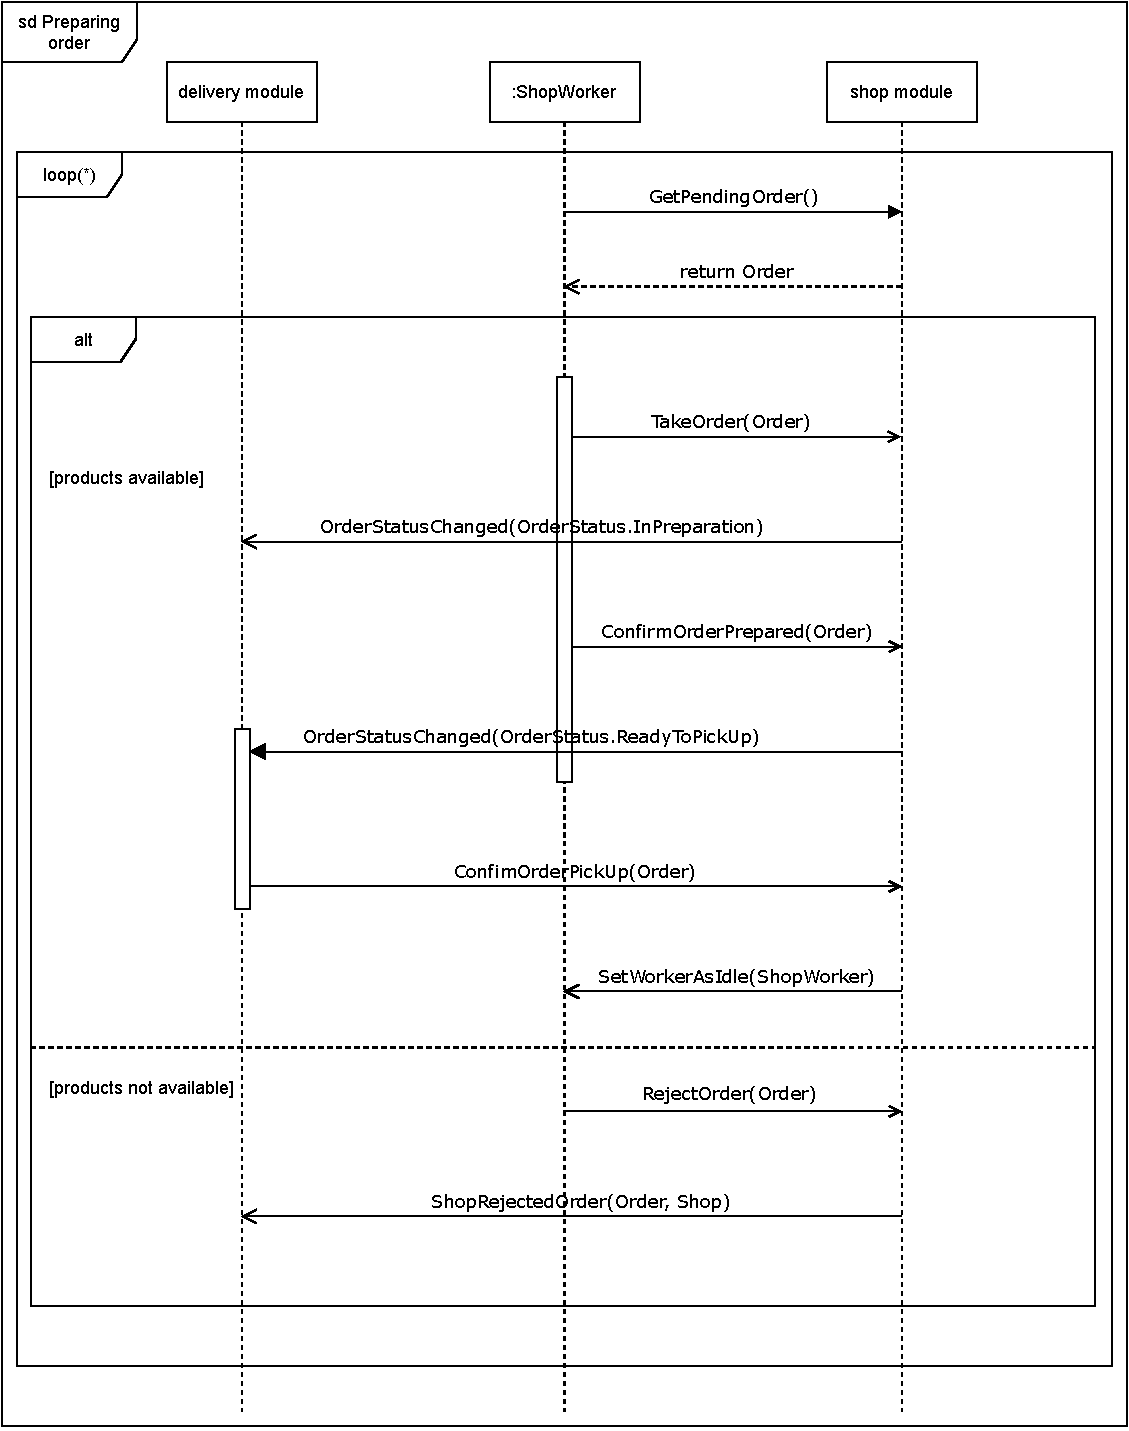
\includegraphics[width=\textwidth]
{diagrams/sequence-diagrams/Shop.pdf}
\end{figure}


\begin{figure}
\caption{Delivery sequence diagram.}
\centering
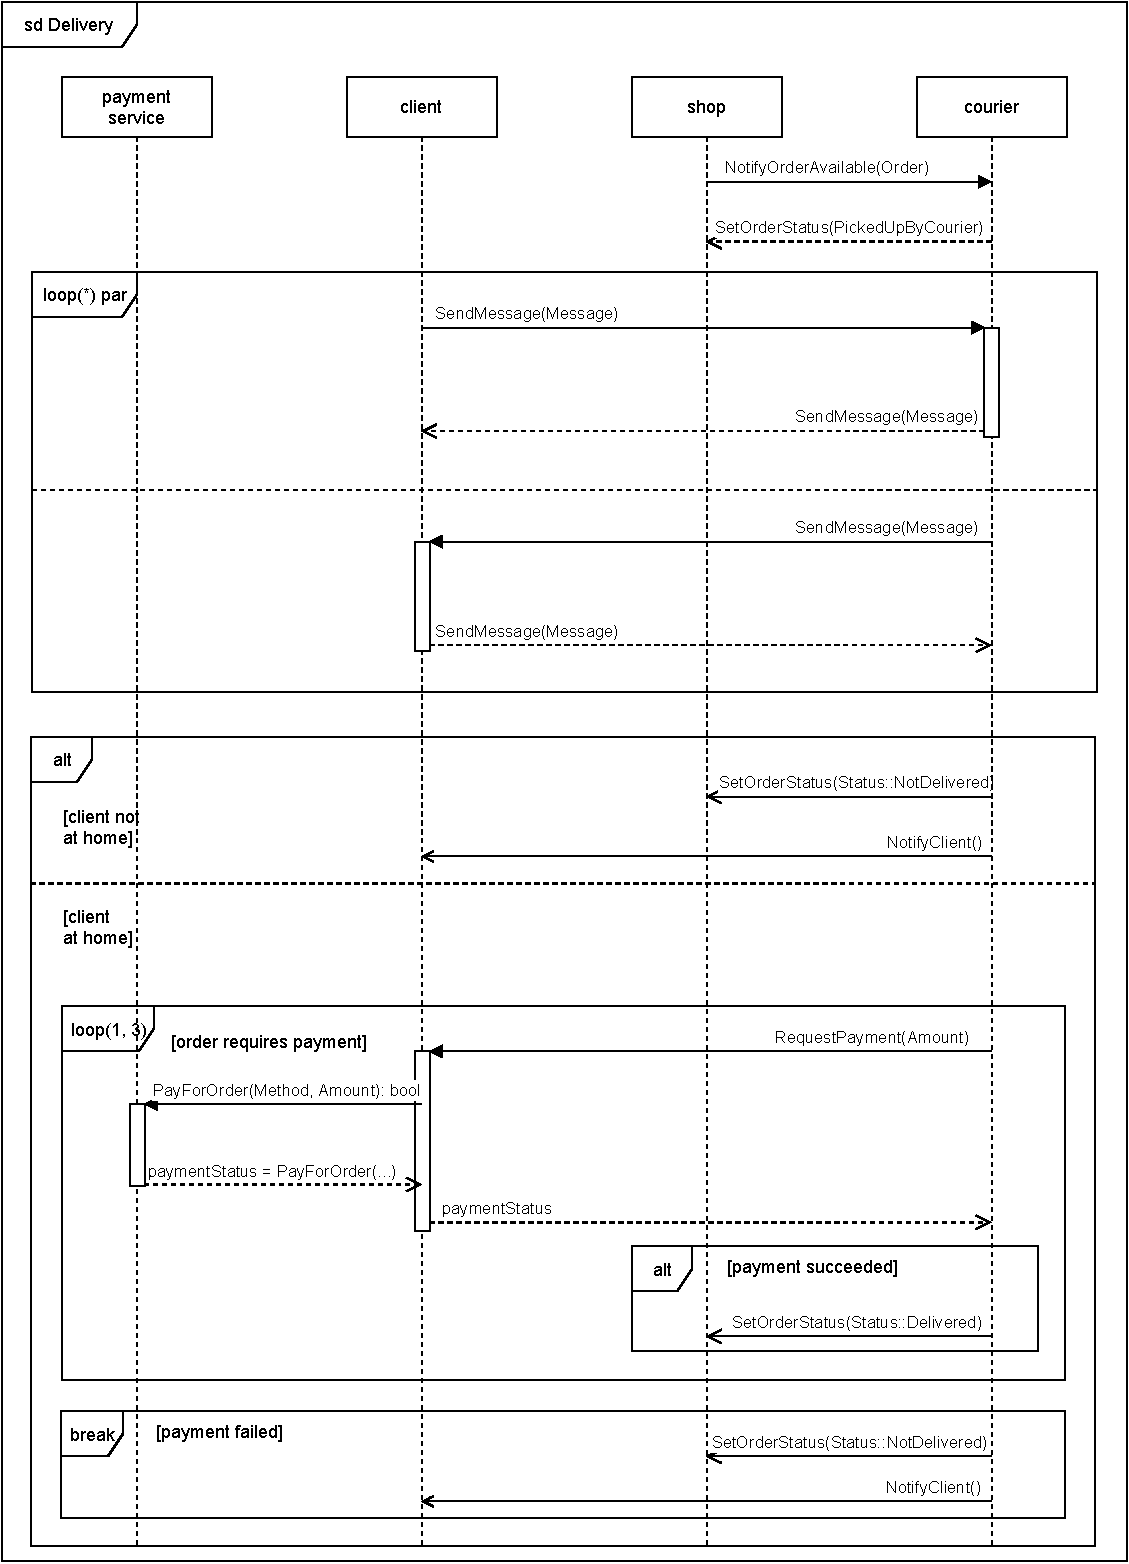
\includegraphics[width=\textwidth]
{diagrams/sequence-diagrams/Courier.pdf}
\end{figure}

\begin{figure}
\caption{Complaint sequence diagram.}
\vspace{5mm}
\centering
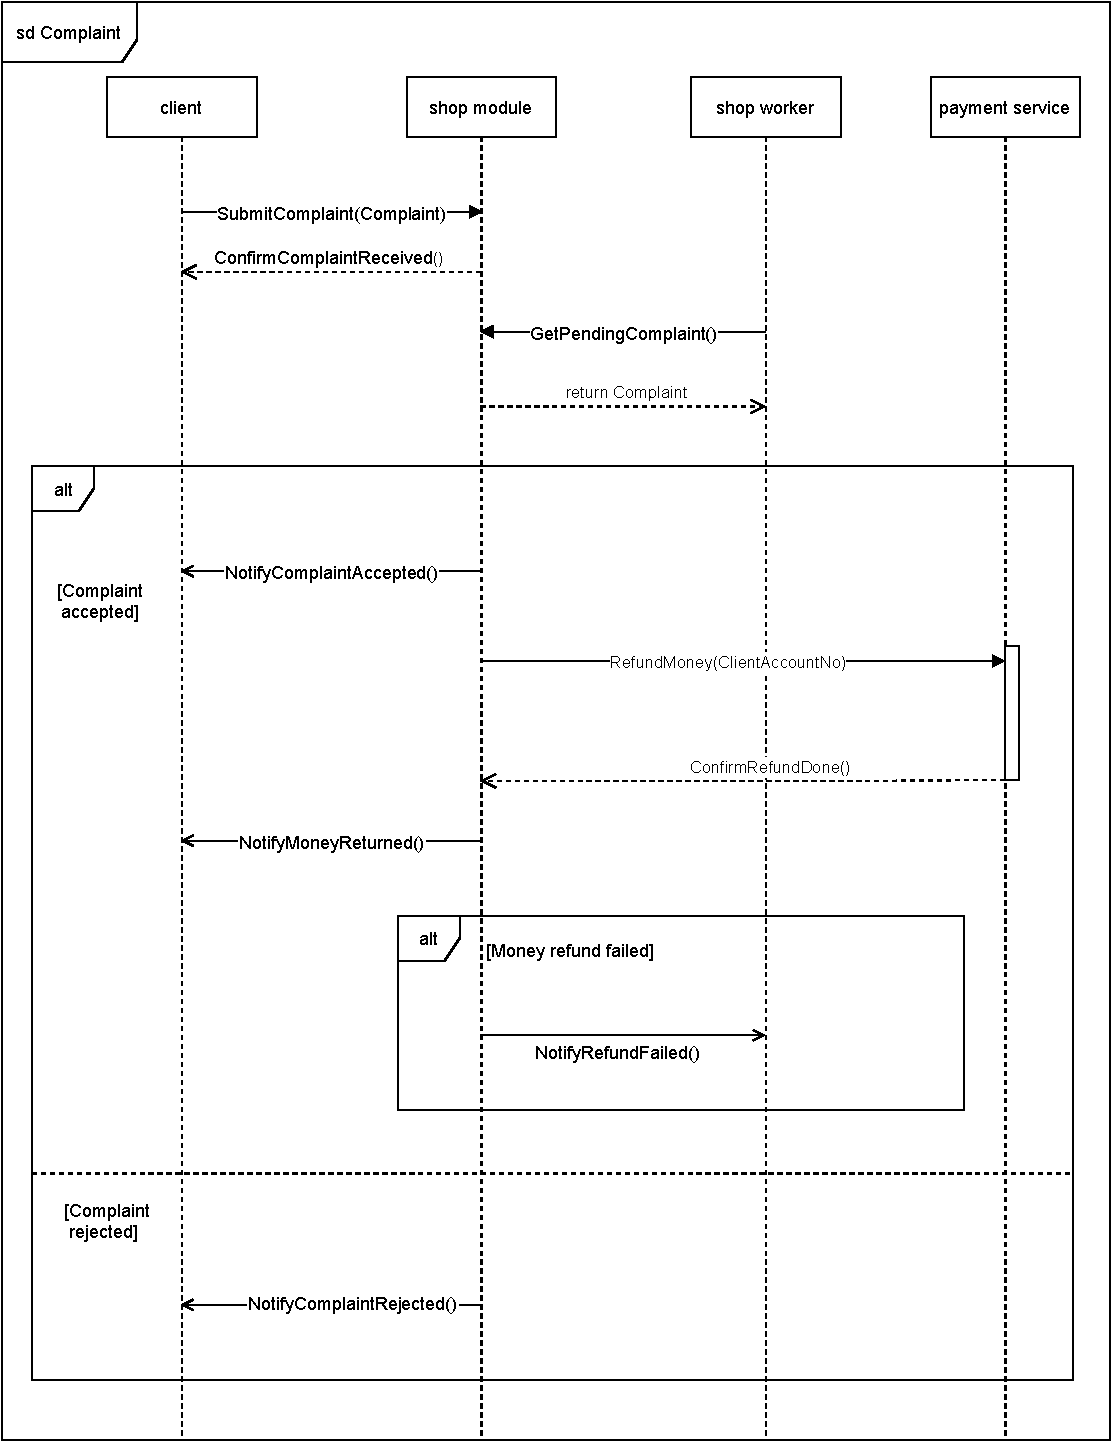
\includegraphics[width=\textwidth]
{diagrams/sequence-diagrams/Complaint.pdf}
\end{figure}



\end{document}